\documentclass[12pt, A4]{article}\usepackage[]{graphicx}\usepackage[]{color}
%% maxwidth is the original width if it is less than linewidth
%% otherwise use linewidth (to make sure the graphics do not exceed the margin)
\makeatletter
\def\maxwidth{ %
  \ifdim\Gin@nat@width>\linewidth
    \linewidth
  \else
    \Gin@nat@width
  \fi
}
\makeatother

\definecolor{fgcolor}{rgb}{0.345, 0.345, 0.345}
\newcommand{\hlnum}[1]{\textcolor[rgb]{0.686,0.059,0.569}{#1}}%
\newcommand{\hlstr}[1]{\textcolor[rgb]{0.192,0.494,0.8}{#1}}%
\newcommand{\hlcom}[1]{\textcolor[rgb]{0.678,0.584,0.686}{\textit{#1}}}%
\newcommand{\hlopt}[1]{\textcolor[rgb]{0,0,0}{#1}}%
\newcommand{\hlstd}[1]{\textcolor[rgb]{0.345,0.345,0.345}{#1}}%
\newcommand{\hlkwa}[1]{\textcolor[rgb]{0.161,0.373,0.58}{\textbf{#1}}}%
\newcommand{\hlkwb}[1]{\textcolor[rgb]{0.69,0.353,0.396}{#1}}%
\newcommand{\hlkwc}[1]{\textcolor[rgb]{0.333,0.667,0.333}{#1}}%
\newcommand{\hlkwd}[1]{\textcolor[rgb]{0.737,0.353,0.396}{\textbf{#1}}}%
\let\hlipl\hlkwb

\usepackage{framed}
\makeatletter
\newenvironment{kframe}{%
 \def\at@end@of@kframe{}%
 \ifinner\ifhmode%
  \def\at@end@of@kframe{\end{minipage}}%
  \begin{minipage}{\columnwidth}%
 \fi\fi%
 \def\FrameCommand##1{\hskip\@totalleftmargin \hskip-\fboxsep
 \colorbox{shadecolor}{##1}\hskip-\fboxsep
     % There is no \\@totalrightmargin, so:
     \hskip-\linewidth \hskip-\@totalleftmargin \hskip\columnwidth}%
 \MakeFramed {\advance\hsize-\width
   \@totalleftmargin\z@ \linewidth\hsize
   \@setminipage}}%
 {\par\unskip\endMakeFramed%
 \at@end@of@kframe}
\makeatother

\definecolor{shadecolor}{rgb}{.97, .97, .97}
\definecolor{messagecolor}{rgb}{0, 0, 0}
\definecolor{warningcolor}{rgb}{1, 0, 1}
\definecolor{errorcolor}{rgb}{1, 0, 0}
\newenvironment{knitrout}{}{} % an empty environment to be redefined in TeX

\usepackage{alltt}
%\usepackage[brazil]{babel}
\usepackage{graphicx}
\usepackage[utf8]{inputenc}
\usepackage[T1]{fontenc}
\usepackage{url}
\usepackage{natbib}
\usepackage{amsmath}
\bibliographystyle{rusnat}
\usepackage{framed, color}
\usepackage{xspace}
\definecolor{shadecolor}{rgb}{0.9, 0.9, 0.9}
\newcommand{\R}{\textnormal{\sffamily\bfseries R}\xspace}
\newcommand{\code}[1]{\texttt{#1}}


\title{Estimates of total tree richness in Amazon - Summary}
\author{Han Ter Steege, Paulo Inácio Prado, Renato Lima, ATDN}
\IfFileExists{upquote.sty}{\usepackage{upquote}}{}
\begin{document}

\maketitle




\section{Data preparation}

\begin{knitrout}
\definecolor{shadecolor}{rgb}{0.969, 0.969, 0.969}\color{fgcolor}\begin{kframe}
\begin{alltt}
\hlstd{dados} \hlkwb{<-} \hlkwd{read.csv2}\hlstd{(}\hlstr{"data.csv"}\hlstd{,} \hlkwc{as.is}\hlstd{=}\hlnum{TRUE}\hlstd{)}
\hlstd{y} \hlkwb{<-} \hlstd{dados}\hlopt{$}\hlstd{N.ind}
\hlstd{Sobs} \hlkwb{<-} \hlkwd{length}\hlstd{(y)}
\hlcom{## Total number of trees (average density x area)}
\hlstd{Tot.t} \hlkwb{<-} \hlnum{567}\hlopt{*}\hlnum{5.5e8}
\hlcom{## Proportion of total trees in the sample}
\hlstd{p1} \hlkwb{<-} \hlkwd{sum}\hlstd{(dados}\hlopt{$}\hlstd{N.ind)}\hlopt{/}\hlstd{Tot.t}
\hlcom{## Total number of plots}
\hlstd{N.plots} \hlkwb{<-} \hlnum{1945}
\hlcom{## Total area hectares}
\hlstd{Tot.A} \hlkwb{<-} \hlnum{5.79e8}
\hlcom{## Sampled area ha}
\hlstd{Samp.A} \hlkwb{<-} \hlnum{2.048e3}
\hlcom{## Amazon RAD sent by Hans}
\hlkwd{load}\hlstd{(}\hlstr{"steege_files/AmazonRAD.RData"}\hlstd{)}
\hlcom{## Truncated Negative binomial }
\hlcom{## (already generated, too slow to rerun)}
\hlstd{nb.pred.full} \hlkwb{<-} \hlkwd{read.csv}\hlstd{(}\hlstr{"NB_RAD.csv"}\hlstd{)}\hlopt{$}\hlstd{x}
\end{alltt}
\end{kframe}
\end{knitrout}

\section{Poisson lognormal}

Seems to overestimate the abundance of the most abundant species (see qq-plots)
 
\begin{knitrout}
\definecolor{shadecolor}{rgb}{0.969, 0.969, 0.969}\color{fgcolor}\begin{kframe}
\begin{alltt}
\hlstd{pln} \hlkwb{<-} \hlkwd{fitpoilog}\hlstd{(y)}
\hlkwd{par}\hlstd{(}\hlkwc{mfrow}\hlstd{=}\hlkwd{c}\hlstd{(}\hlnum{2}\hlstd{,}\hlnum{2}\hlstd{))}
\hlkwd{plot}\hlstd{(pln)}
\hlkwd{par}\hlstd{(}\hlkwc{mfrow}\hlstd{=}\hlkwd{c}\hlstd{(}\hlnum{1}\hlstd{,}\hlnum{1}\hlstd{))}
\end{alltt}
\end{kframe}

{\centering 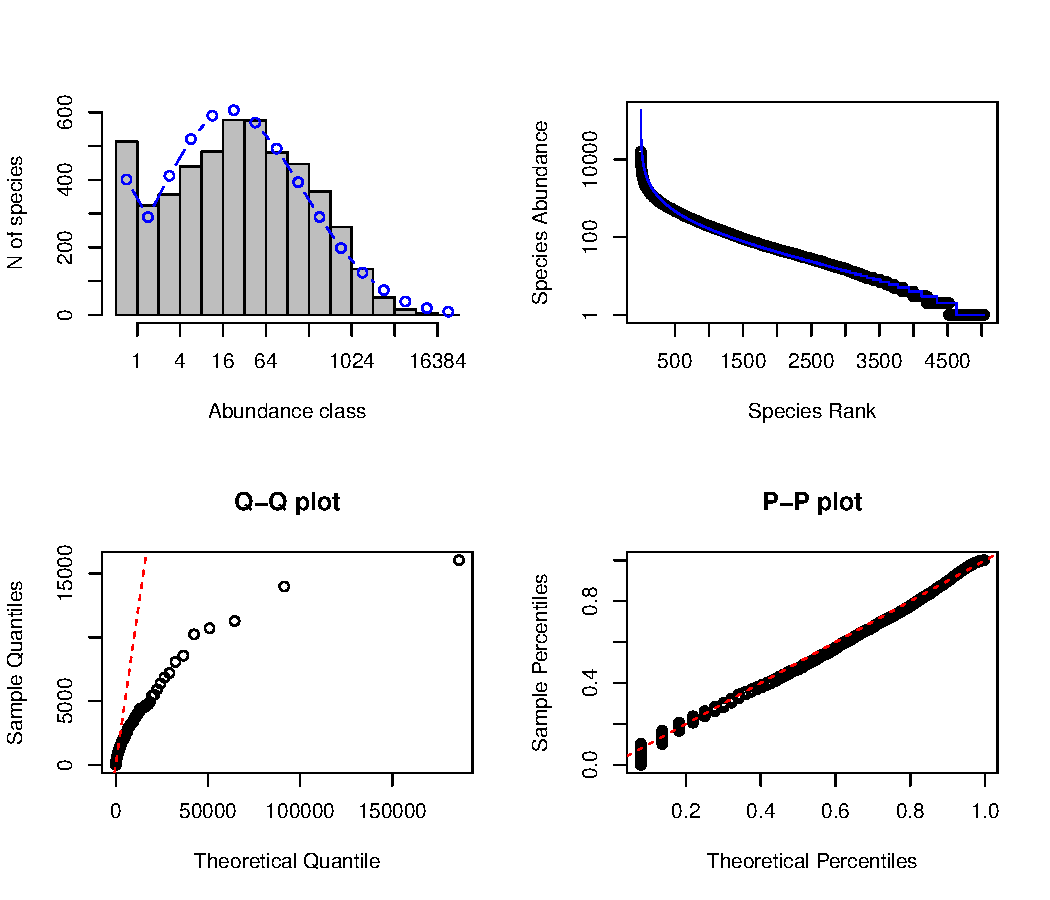
\includegraphics[width=\maxwidth]{figure/fit_pln-1} 

}



\end{knitrout}


\subsection*{Estimating species richness from PLN}

The fitted PLN allows to estimate the probability value assigned to species that
had zero abundance in the sample:

\begin{knitrout}
\definecolor{shadecolor}{rgb}{0.969, 0.969, 0.969}\color{fgcolor}\begin{kframe}
\begin{alltt}
\hlstd{(pln.d0} \hlkwb{<-} \hlkwd{dpoilog}\hlstd{(}\hlnum{0}\hlstd{,} \hlkwc{mu} \hlstd{= pln.cf[}\hlnum{1}\hlstd{],} \hlkwc{sig}\hlstd{=pln.cf[}\hlnum{2}\hlstd{]))}
\end{alltt}
\begin{verbatim}
## [1] 0.1120095
\end{verbatim}
\end{kframe}
\end{knitrout}

That is, an estimate that the recorded species are 89\%
of the total number of species.
This gives an estimate of 5668 species.


\section{Log-series}

Log-series seems to overestimate the number of singletons
and to underestimate the abundance of species with intermediary abundances
(between 16 and 64 individuals, see octave plot). Also, the qq-plot shows that
the model underestimates the larger abundances.

 
\begin{knitrout}
\definecolor{shadecolor}{rgb}{0.969, 0.969, 0.969}\color{fgcolor}\begin{kframe}
\begin{alltt}
\hlstd{y.ls} \hlkwb{<-} \hlkwd{fitls}\hlstd{(y)}
\hlkwd{par}\hlstd{(}\hlkwc{mfrow}\hlstd{=}\hlkwd{c}\hlstd{(}\hlnum{2}\hlstd{,}\hlnum{2}\hlstd{))}
\hlkwd{plot}\hlstd{(y.ls)}
\hlkwd{par}\hlstd{(}\hlkwc{mfrow}\hlstd{=}\hlkwd{c}\hlstd{(}\hlnum{1}\hlstd{,}\hlnum{1}\hlstd{))}
\end{alltt}
\end{kframe}

{\centering 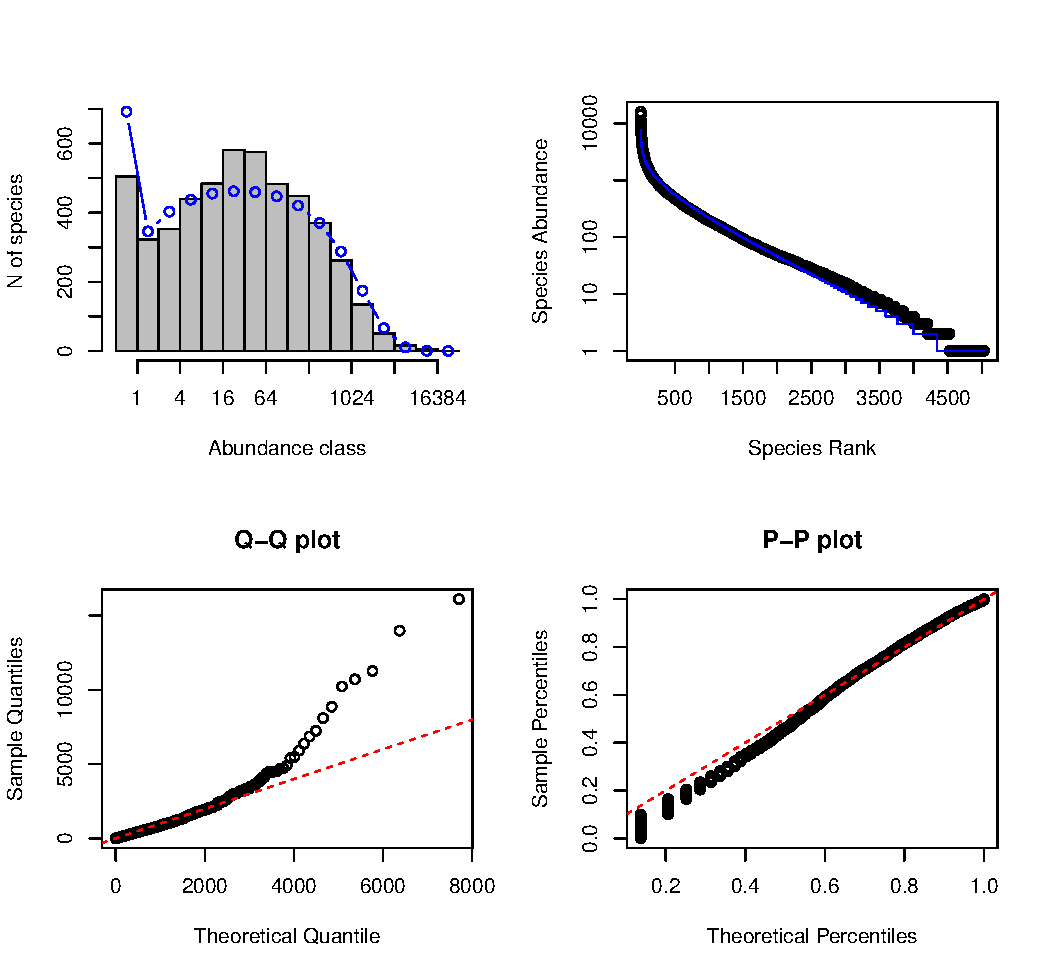
\includegraphics[width=\maxwidth]{figure/fit_ls-1} 

}



\end{knitrout}

\subsection*{Estimate of species richness}

From the value of $\alpha$ estimated from the sample of plots:
 
\begin{knitrout}
\definecolor{shadecolor}{rgb}{0.969, 0.969, 0.969}\color{fgcolor}\begin{kframe}
\begin{alltt}
\hlstd{alpha} \hlkwb{<-} \hlkwd{coef}\hlstd{(y.ls)[[}\hlnum{2}\hlstd{]]}
\hlstd{(S.ls} \hlkwb{<-} \hlstd{alpha}\hlopt{*}\hlkwd{log}\hlstd{(}\hlnum{1} \hlopt{+} \hlstd{Tot.t}\hlopt{/}\hlstd{alpha))}
\end{alltt}
\begin{verbatim}
## [1] 13809.86
\end{verbatim}
\end{kframe}
\end{knitrout}

And here is the confidence interval for Fisher's $\alpha$ and the
interval for estimated total richness from these values

\begin{knitrout}
\definecolor{shadecolor}{rgb}{0.969, 0.969, 0.969}\color{fgcolor}\begin{kframe}
\begin{alltt}
\hlstd{(ls.ci} \hlkwb{<-} \hlkwd{confint}\hlstd{(y.ls))}
\end{alltt}
\begin{verbatim}
##    2.5 %   97.5 % 
## 638.9166 750.1000
\end{verbatim}
\begin{alltt}
\hlcom{## Estimated species richness for lower bound of alpha's IC}
\hlstd{ls.ci[}\hlnum{1}\hlstd{]}\hlopt{*}\hlkwd{log}\hlstd{(}\hlnum{1} \hlopt{+} \hlstd{Tot.t}\hlopt{/}\hlstd{ls.ci[}\hlnum{1}\hlstd{])}
\end{alltt}
\begin{verbatim}
##    2.5 % 
## 12782.17
\end{verbatim}
\begin{alltt}
\hlstd{ls.ci[}\hlnum{2}\hlstd{]}\hlopt{*}\hlkwd{log}\hlstd{(}\hlnum{1} \hlopt{+} \hlstd{Tot.t}\hlopt{/}\hlstd{ls.ci[}\hlnum{2}\hlstd{])}
\end{alltt}
\begin{verbatim}
##   97.5 % 
## 14886.17
\end{verbatim}
\end{kframe}
\end{knitrout}

\section{Zero-truncated Negative binomial}
\label{sec:negbin}

Here I use the method proposed by \citet{tovo2017}. The first step is
to fit a zero-truncated negative binomial (TNB) to the abundances in the sample.
I did that with the \emph{VGAM} package (as the authors did)
and also with the \emph{sads} package. 
The results were similar, and the fit looks identical to
those provided by the log-series (but has much lower AIC value, see below).
 
\begin{knitrout}
\definecolor{shadecolor}{rgb}{0.969, 0.969, 0.969}\color{fgcolor}\begin{kframe}
\begin{alltt}
\hlcom{## With VGAM}
\hlstd{y.nb} \hlkwb{<-} \hlkwd{vglm}\hlstd{(y} \hlopt{~} \hlnum{1}\hlstd{, posnegbinomial)}
\hlcom{## With sads}
\hlstd{y.nb2} \hlkwb{<-} \hlkwd{fitnbinom}\hlstd{(y,} \hlkwc{start.value}\hlstd{=}\hlkwd{c}\hlstd{(}\hlkwc{size}\hlstd{=}\hlnum{0.3}\hlstd{,} \hlkwc{mu}\hlstd{=}\hlkwd{mean}\hlstd{(y)))}
\hlcom{## Comparing: }
\hlkwd{exp}\hlstd{(}\hlkwd{coef}\hlstd{(y.nb))}
\end{alltt}
\begin{verbatim}
## (Intercept):1 (Intercept):2 
##   48.96347392    0.04048581
\end{verbatim}
\begin{alltt}
\hlkwd{coef}\hlstd{(y.nb2)}
\end{alltt}
\begin{verbatim}
##        size          mu 
##  0.04153996 50.08844429
\end{verbatim}
\end{kframe}
\end{knitrout}

\begin{knitrout}
\definecolor{shadecolor}{rgb}{0.969, 0.969, 0.969}\color{fgcolor}\begin{kframe}
\begin{alltt}
\hlkwd{par}\hlstd{(}\hlkwc{mfrow}\hlstd{=}\hlkwd{c}\hlstd{(}\hlnum{2}\hlstd{,}\hlnum{2}\hlstd{))}
\hlkwd{plot}\hlstd{(y.nb2)}
\hlkwd{par}\hlstd{(}\hlkwc{mfrow}\hlstd{=}\hlkwd{c}\hlstd{(}\hlnum{1}\hlstd{,}\hlnum{1}\hlstd{))}
\end{alltt}
\end{kframe}

{\centering 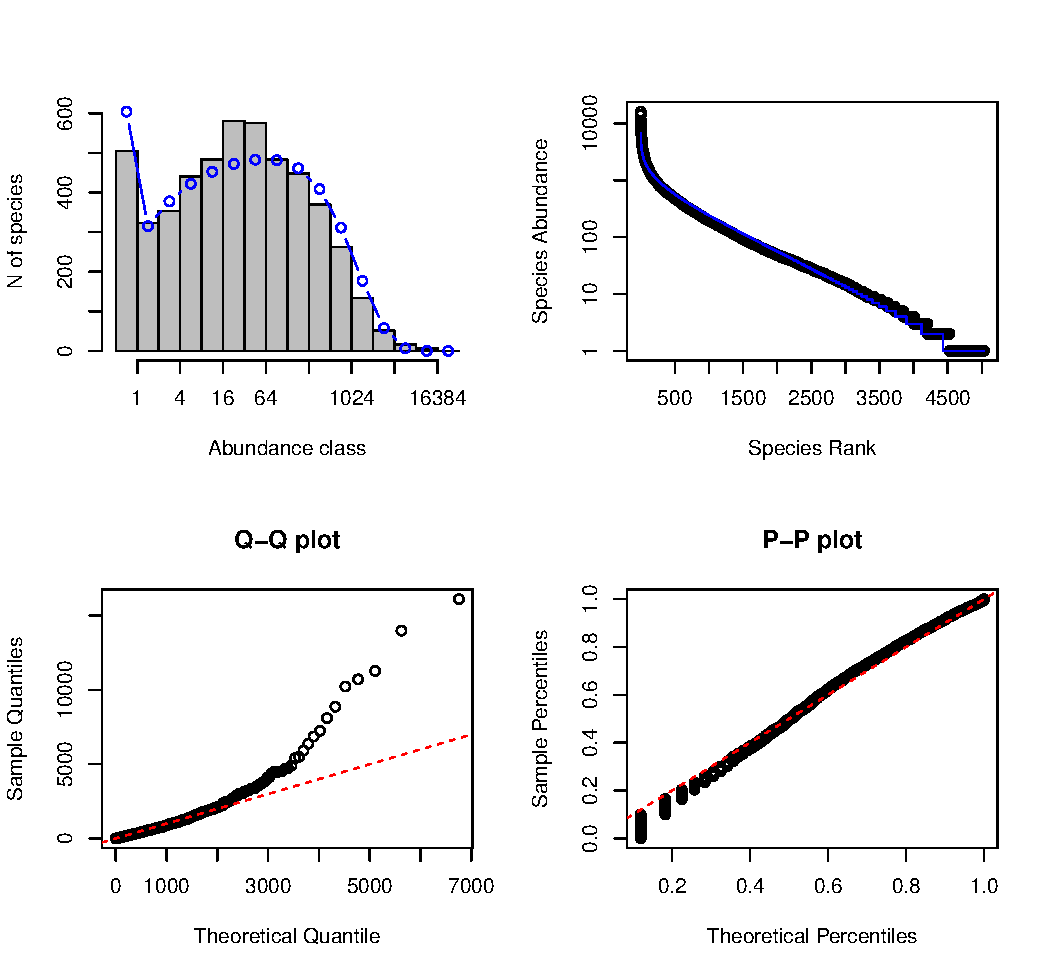
\includegraphics[width=\maxwidth]{figure/nb_plots-1} 

}



\end{knitrout}


\subsection*{Estimate of  species richness}

Following the recipe of \citet{tovo2017}:

 
\begin{knitrout}
\definecolor{shadecolor}{rgb}{0.969, 0.969, 0.969}\color{fgcolor}\begin{kframe}
\begin{alltt}
\hlstd{cf.nb} \hlkwb{<-} \hlkwd{coef}\hlstd{(y.nb2)}
\hlstd{csi.p} \hlkwb{<-} \hlkwd{unname}\hlstd{(cf.nb[}\hlnum{2}\hlstd{]}\hlopt{/}\hlstd{(}\hlkwd{sum}\hlstd{(cf.nb)))}
\hlstd{csi} \hlkwb{<-} \hlstd{csi.p}\hlopt{/}\hlstd{(p1}\hlopt{+}\hlstd{(}\hlnum{1}\hlopt{-}\hlstd{p1)}\hlopt{*}\hlstd{csi.p)}
\hlcom{## Estimated number of species }
\hlstd{S.nb} \hlkwb{<-} \hlstd{Sobs}\hlopt{*}\hlstd{(}\hlnum{1}\hlopt{-}\hlstd{(}\hlnum{1}\hlopt{-}\hlstd{csi)}\hlopt{^}\hlstd{cf.nb[}\hlnum{1}\hlstd{])} \hlopt{/} \hlstd{(}\hlnum{1}\hlopt{-}\hlstd{(}\hlnum{1}\hlopt{-}\hlstd{csi.p)}\hlopt{^}\hlstd{cf.nb[}\hlnum{1}\hlstd{])}
\hlstd{(S.nb} \hlkwb{<-} \hlkwd{unname}\hlstd{(S.nb))}
\end{alltt}
\begin{verbatim}
## [1] 11038.67
\end{verbatim}
\end{kframe}
\end{knitrout}

I did a simple function to automate the calculations and to return
the confidence intervals, based on the confidence intervals of the 
coefficients of the NB fit (see file \code{functions.R})

 
\begin{knitrout}
\definecolor{shadecolor}{rgb}{0.969, 0.969, 0.969}\color{fgcolor}\begin{kframe}
\begin{alltt}
\hlstd{(tovo.S} \hlkwb{<-} \hlkwd{tovo}\hlstd{(}\hlkwc{fit} \hlstd{= y.nb2,} \hlkwc{p} \hlstd{= p1,} \hlkwc{CI}\hlstd{=}\hlnum{TRUE}\hlstd{))}
\end{alltt}
\begin{verbatim}
## Estimated species richness: 11038.67 
##  95% CI: 2.73884e-09 - 2.480429e-09
## $S.est
## [1] 11038.67
## 
## $CIs
##              2.5 %       97.5 %
## size  2.547345e-02 5.566008e-02
## mu    3.248973e+01 6.429281e+01
## prob  2.480429e-09 2.738840e-09
## S.est 1.206354e+04 1.027710e+04
\end{verbatim}
\end{kframe}
\end{knitrout}


\section{Model selection}

Among the three models, TNB
provides the best fit to the abundances in the sample:

 
\begin{knitrout}
\definecolor{shadecolor}{rgb}{0.969, 0.969, 0.969}\color{fgcolor}\begin{kframe}
\begin{alltt}
\hlkwd{AICtab}\hlstd{(pln, y.nb2, y.ls,} \hlkwc{base}\hlstd{=}\hlnum{TRUE}\hlstd{)}
\end{alltt}
\begin{verbatim}
##       AIC     dAIC    df
## y.nb2 54530.9     0.0 2 
## y.ls  54557.5    26.6 1 
## pln   54577.6    46.6 2
\end{verbatim}
\end{kframe}
\end{knitrout}

TNB overestimates the higher abundances, while the logseries
underestimates the lower abundances in the sample:

\begin{knitrout}
\definecolor{shadecolor}{rgb}{0.969, 0.969, 0.969}\color{fgcolor}

{\centering \includegraphics[width=\maxwidth]{figure/Comparing_LS_and_NB-1} 

}



\end{knitrout}

\section{Estimates based in the regional RAD}

\subsection*{Linear extrapolation from the regional RAD}

Here I replicated the extrapolation method from the regional RAD of the
estimated abundances for the whole Amazonia, first for the logseries projection:

\begin{knitrout}
\definecolor{shadecolor}{rgb}{0.969, 0.969, 0.969}\color{fgcolor}\begin{kframe}
\begin{alltt}
\hlcom{## Regional RAD}
\hlstd{pop.rad} \hlkwb{<-} \hlkwd{rad}\hlstd{(dados}\hlopt{$}\hlstd{population)}
\hlcom{## Linear regression through central 50% quantiles of the RAD}
\hlstd{p.lm} \hlkwb{<-} \hlkwd{lm}\hlstd{(}\hlkwd{log}\hlstd{(abund)}\hlopt{~}\hlstd{rank,} \hlkwc{data}\hlstd{=}\hlkwd{data.frame}\hlstd{(pop.rad),}
           \hlkwc{subset}\hlstd{=rank}\hlopt{>}\hlkwd{max}\hlstd{(rank)}\hlopt{*}\hlnum{.25}\hlopt{&}\hlstd{rank}\hlopt{<}\hlkwd{max}\hlstd{(rank)}\hlopt{*}\hlnum{.75}\hlstd{)}
\hlcom{## Regression coefficients}
\hlstd{cf.p.lm} \hlkwb{<-} \hlkwd{unname}\hlstd{(}\hlkwd{coef}\hlstd{(p.lm))}
\hlcom{## Logseries projection (upper bound)}
\hlstd{(S.reg1} \hlkwb{<-} \hlkwd{abs}\hlstd{(cf.p.lm[}\hlnum{1}\hlstd{]}\hlopt{/}\hlstd{cf.p.lm[}\hlnum{2}\hlstd{]))}
\end{alltt}
\begin{verbatim}
## [1] 15279.03
\end{verbatim}
\end{kframe}
\end{knitrout}

Which is exactly the value reported in the manuscript (\ensuremath{1.5279\times 10^{4}} species). 

According to \citet{ulrich2005}, this is an upper limit to the estimation of species. 
They propose that the same linear extrapolation assuming a log-normal is a lower-bound estimate.
Following their recipe (eq.2) such lower bound would be:

\begin{knitrout}
\definecolor{shadecolor}{rgb}{0.969, 0.969, 0.969}\color{fgcolor}\begin{kframe}
\begin{alltt}
\hlstd{d} \hlkwb{<-} \hlkwd{log}\hlstd{(}\hlkwd{max}\hlstd{(dados}\hlopt{$}\hlstd{population))}\hlopt{-}\hlstd{cf.p.lm[}\hlnum{1}\hlstd{]}
\hlstd{(S.reg2} \hlkwb{<-} \hlkwd{abs}\hlstd{((cf.p.lm[}\hlnum{1}\hlstd{]}\hlopt{-}\hlstd{d)}\hlopt{/}\hlstd{cf.p.lm[}\hlnum{2}\hlstd{]))}
\end{alltt}
\begin{verbatim}
## [1] 12791.71
\end{verbatim}
\end{kframe}
\end{knitrout}

\subsection*{Regional RAD from TNB}

Here I compare the regional RAD with RADs predicted  by 
the zero-truncated negative binomial and the upper-bound and lower-bound estimate of species
obtained above.

The RAD of negative binomial was upscaled according to \citep{tovo2017} 
and gets to the number of species estimated by this method (section~\ref{sec:negbin}).

\begin{knitrout}
\definecolor{shadecolor}{rgb}{0.969, 0.969, 0.969}\color{fgcolor}

{\centering \includegraphics[width=\maxwidth]{figure/nbinom_rad-1} 

}



\end{knitrout}

The blue line is the RAD predicted by zero-truncated negative binomial upscaled to the total number of
trees in Amazonia. %Broken lines are approximated 95\% CIs. 
The red line is the upscaled log-series for the Amazon,
as sent by Hans ( file \code{script\_for\_Paulo.R} ). 
Black lines are the linear extrapolations for the 50\% 
central quantile of the estimated population sizes, for
the Log-series and log-normal model \citep{ulrich2005}.

The negative binomial has a power-bending factor that
results in a lower estimate of total richness, below to
the lower-limit of the linear extrapolations.

\section{Comparing population sizes predicted by LS and NB regional RADs}

\subsection*{Methods}

To check which RAD model would approximate better the total population sizes estimated
for the sampled species, we simulated samples from the Amazon RAD generated by the Log-series 
and Truncated Negative Binomial, with and without clumping. 
In both cases we assumed a random drawn of 1945 1-ha plots
from the Amazon RADs, where the number of individuals of each species
in each plot followed a Poisson (random sampling) or a Negative Binomial (clumped sampling)
distribution. 

The simulated population sizes where the total population sizes taken from
the regional RAD, only for those species that had been recorded 
in the simulated sample. 
The probability of each species be not included in a sample of $N$ plots is  $P(0)=(1-p)^N$.

Where $p$ is the probability of occurrence in each plot. 
Given the density of the species per plot $\mu$, 
for a Poisson sample 

\begin{equation}
  \label{eq:3}
  P(0) = e^{-\mu} 
\end{equation} 

and for a Negative Binomial sample

\begin{equation}
  \label{eq:2}
  P(0) = \left( \frac{k}{k+\mu} \right)^k 
\end{equation}

Where $k$ is the dispersion parameter of the negative binomial distribution.
%This coefficient adds extra variance compared to a Poisson sampling.
Thus we simulated occurrences of each species by sampling presence/absences
from a Bernoulli distribution with probability of occurrence $1-P(0)$.

\subsubsection*{Simulating clumping coefficients}

For simulations of clumped sampling, 
we allowed interspecific variation in clumping, 
by allowing a different value of the dispersion coefficient ($k$) for each species.
Hence, we had to define the value of $k$ for each species in the regional
RADs. We did that by (i) estimating the values of $k$ for the sampled species and
then (ii) by using the relationship between $k$ and $\mu$ to estimate the values of $k$
of each species.

To estimate the values of the aggregation coefficients
of the sampled species
we assumed that the number of plots that each species has been recorded follows
a binomial distribution with a probability of occurrence in each plot of $p=1-P(0)$,
with $P(0)$ from equation~\ref{eq:2}.
The parameter $k$ was then estimated by numerically maximizing the
log-likelihood function of the binomial distribution:

\begin{equation}
  \mathcal{L}(k | \mu, N, f_0) \ =  \ f_0 \ln (1-p) + (N - f_0) \ln p
\end{equation}

Where $N$ is the total number of plots, $f_0$ is 
the number of plots where the species was not recorded.
This log-likelihood function is conditioned to $\mu$, because this parameter was 
set to the observed density of each species in the sample.

Once we estimated a value of $k$ for each species recorded, 
we fit a linear regression of these values in function of the
observed species densities, in log scale.
The commands and model summary were:

\begin{knitrout}
\definecolor{shadecolor}{rgb}{0.969, 0.969, 0.969}\color{fgcolor}\begin{kframe}
\begin{alltt}
\hlcom{## estimating k parameter of a NB for each species }
\hlstd{dados}\hlopt{$}\hlstd{dens.ha} \hlkwb{<-} \hlstd{dados}\hlopt{$}\hlstd{N.ind}\hlopt{/}\hlstd{Samp.A}
\hlstd{dados}\hlopt{$}\hlstd{k} \hlkwb{<-} \hlkwd{est.kv}\hlstd{(}\hlkwc{mu}\hlstd{=dados}\hlopt{$}\hlstd{dens.ha,}
                  \hlkwc{nzeroes}\hlstd{=N.plots}\hlopt{-}\hlstd{dados}\hlopt{$}\hlstd{N.plots,}
                  \hlkwc{Nplots}\hlstd{=N.plots)}
\hlstd{lm.k} \hlkwb{<-}\hlkwd{lm}\hlstd{(}\hlkwd{log}\hlstd{(k)}\hlopt{~}\hlkwd{log}\hlstd{(dens.ha),}
          \hlkwc{data}\hlstd{=dados,} \hlkwc{subset}\hlstd{=k}\hlopt{<}\hlnum{1}\hlstd{)}
\hlcom{## Estimated regression standard error}
\hlstd{lm.k.sigma} \hlkwb{<-} \hlkwd{summary}\hlstd{(lm.k)}\hlopt{$}\hlstd{sigma}
\hlkwd{summary}\hlstd{(lm.k)}
\end{alltt}
\begin{verbatim}
## 
## Call:
## lm(formula = log(k) ~ log(dens.ha), data = dados, subset = k < 
##     1)
## 
## Residuals:
##     Min      1Q  Median      3Q     Max 
## -5.3919 -0.6511  0.1124  0.8366  5.1195 
## 
## Coefficients:
##              Estimate Std. Error t value Pr(>|t|)    
## (Intercept)  -3.09985    0.04425  -70.05   <2e-16 ***
## log(dens.ha)  0.59138    0.01067   55.42   <2e-16 ***
## ---
## Signif. codes:  0 '***' 0.001 '**' 0.01 '*' 0.05 '.' 0.1 ' ' 1
## 
## Residual standard error: 1.236 on 4187 degrees of freedom
## Multiple R-squared:  0.4231,	Adjusted R-squared:  0.423 
## F-statistic:  3071 on 1 and 4187 DF,  p-value: < 2.2e-16
\end{verbatim}
\end{kframe}
\end{knitrout}

And a plot of with the regression line is

\begin{knitrout}
\definecolor{shadecolor}{rgb}{0.969, 0.969, 0.969}\color{fgcolor}

{\centering \includegraphics[width=\maxwidth]{figure/lok_k_x_log_density_plot-1} 

}



\end{knitrout}

We then used this regression model to set a value of $k$ for each species from
their abundances as predicted by the regional RAD. 
In each simulation we drawn a value of $\ln k$ for each species
in the Amazon RAD from a Normal distribution with the mean as
the predicted value from the linear regression above for the population
density of the species in the RAD. The standard deviation of these
Normal distributions was the standard error of the linear regression.

\subsubsection*{Simulation scripts}

\begin{knitrout}
\definecolor{shadecolor}{rgb}{0.969, 0.969, 0.969}\color{fgcolor}\begin{kframe}
\begin{alltt}
\hlcom{## Simulation of population sizes from samples of }
\hlcom{## the regional RADs}
\hlstd{nrep} \hlkwb{<-} \hlnum{100} \hlcom{#number of repetitions}
\hlcom{## Samples from LS RAD}
\hlcom{## Matrices to store samples}
\hlstd{tmp1} \hlkwb{<-} \hlstd{tmp2} \hlkwb{<-} \hlkwd{matrix}\hlstd{(}\hlnum{0}\hlstd{,}\hlkwc{nrow}\hlstd{=}\hlkwd{length}\hlstd{(Amazon.rad),} \hlkwc{ncol}\hlstd{=nrep)}
\hlkwa{for}\hlstd{(j} \hlkwa{in} \hlnum{1}\hlopt{:}\hlstd{nrep)\{}
    \hlcom{## Samples aggregation parameters for each species according to }
    \hlcom{## the linear model + standard errors of this model}
    \hlstd{k1} \hlkwb{<-} \hlkwd{exp}\hlstd{(}\hlkwd{rnorm}\hlstd{(}\hlkwd{length}\hlstd{(Amazon.rad),}
                    \hlkwc{mean}\hlstd{=Amazon.rad.lk,} \hlkwc{sd}\hlstd{=lm.k.sigma))}
    \hlcom{## Random (Poisson) sample}
    \hlstd{y1} \hlkwb{<-} \hlkwd{mapply}\hlstd{(sim.occ,} \hlkwc{mu} \hlstd{= Amazon.rad}\hlopt{/}\hlstd{Tot.A,}
                   \hlkwc{MoreArgs}\hlstd{=}\hlkwd{list}\hlstd{(}\hlkwc{N} \hlstd{= N.plots))}
    \hlcom{## Clumped (negative binomial) sample}
    \hlstd{y2} \hlkwb{<-} \hlkwd{mapply}\hlstd{(sim.occ,} \hlkwc{mu} \hlstd{= Amazon.rad}\hlopt{/}\hlstd{Tot.A,} \hlkwc{size} \hlstd{= k1,}
                   \hlkwc{MoreArgs}\hlstd{=}\hlkwd{list}\hlstd{(}\hlkwc{N} \hlstd{= N.plots,} \hlkwc{pois.samp}\hlstd{=}\hlnum{FALSE}\hlstd{))}
    \hlcom{## Pick the population sizes for species}
    \hlcom{## recorded in the sample}
    \hlstd{tmp1[}\hlnum{1}\hlopt{:}\hlkwd{sum}\hlstd{(y1),j]} \hlkwb{<-} \hlstd{Amazon.rad[y1}\hlopt{>}\hlnum{0}\hlstd{]}
    \hlstd{tmp2[}\hlnum{1}\hlopt{:}\hlkwd{sum}\hlstd{(y2),j]} \hlkwb{<-} \hlstd{Amazon.rad[y2}\hlopt{>}\hlnum{0}\hlstd{]}
\hlstd{\}}
\hlcom{## Simulation of samples from TNB }
\hlstd{tmp4} \hlkwb{<-} \hlstd{tmp3} \hlkwb{<-} \hlkwd{matrix}\hlstd{(}\hlnum{0}\hlstd{,}\hlkwc{nrow}\hlstd{=}\hlkwd{length}\hlstd{(nb.pred.full),} \hlkwc{ncol}\hlstd{=nrep)}
\hlkwa{for}\hlstd{(j} \hlkwa{in} \hlnum{1}\hlopt{:}\hlstd{nrep)\{}
    \hlstd{k2} \hlkwb{<-} \hlkwd{exp}\hlstd{(}\hlkwd{rnorm}\hlstd{(}\hlkwd{length}\hlstd{(nb.pred.full),}
                    \hlkwc{mean}\hlstd{=nb.pred.full.lk,} \hlkwc{sd}\hlstd{=lm.k.sigma))}
    \hlstd{y3} \hlkwb{<-} \hlkwd{mapply}\hlstd{(sim.occ,} \hlkwc{mu} \hlstd{= nb.pred.full}\hlopt{/}\hlstd{Tot.A,}
                   \hlkwc{MoreArgs}\hlstd{=}\hlkwd{list}\hlstd{(}\hlkwc{N} \hlstd{= N.plots))}
    \hlstd{y4} \hlkwb{<-} \hlkwd{mapply}\hlstd{(sim.occ,} \hlkwc{mu} \hlstd{= nb.pred.full}\hlopt{/}\hlstd{Tot.A,} \hlkwc{size} \hlstd{= k2,}
                   \hlkwc{MoreArgs}\hlstd{=}\hlkwd{list}\hlstd{(}\hlkwc{N} \hlstd{= N.plots,} \hlkwc{pois.samp}\hlstd{=}\hlnum{FALSE}\hlstd{))}
    \hlstd{tmp3[}\hlnum{1}\hlopt{:}\hlkwd{sum}\hlstd{(y3),j]} \hlkwb{<-} \hlstd{nb.pred.full[y3}\hlopt{>}\hlnum{0}\hlstd{]}
    \hlstd{tmp4[}\hlnum{1}\hlopt{:}\hlkwd{sum}\hlstd{(y4),j]} \hlkwb{<-} \hlstd{nb.pred.full[y4}\hlopt{>}\hlnum{0}\hlstd{]}
\hlstd{\}}
\hlcom{## Mean RADs for each simulation}
\hlstd{ls.rnd} \hlkwb{<-} \hlkwd{apply}\hlstd{(tmp1,}\hlnum{1}\hlstd{,mean)}
\hlstd{ls.clump} \hlkwb{<-} \hlkwd{apply}\hlstd{(tmp2,}\hlnum{1}\hlstd{,mean)}
\hlstd{nb.rnd} \hlkwb{<-} \hlkwd{apply}\hlstd{(tmp3,}\hlnum{1}\hlstd{,mean)}
\hlstd{nb.clump} \hlkwb{<-} \hlkwd{apply}\hlstd{(tmp4,}\hlnum{1}\hlstd{,mean)}
\end{alltt}
\end{kframe}
\end{knitrout}


\subsubsection*{Results}

Visually, clumped sample from a LS RAD and random (Poisson) sampling
from a TNB RAD approximate better the total population sizes:

\begin{knitrout}
\definecolor{shadecolor}{rgb}{0.969, 0.969, 0.969}\color{fgcolor}

{\centering \includegraphics[width=\maxwidth]{figure/plot_sampled_RADS-1} 

}



\end{knitrout}


The aggregation coefficients estimated from the sample clearly show that
the species are clumped accross 1-ha plots, and so that
Poisson sampling is not realistic. This would suffice to
discard the TNB RAD, as they only provides a realistic fit under Poisson sampling.
Moreover, the mean-squared errors of the log of simulated values relative
to the log of the estimated population sizes clearly show that
the clumped sample of LS is a best approximation, among those tested:


% latex table generated in R 3.5.1 by xtable 1.8-2 package
% Sat Dec  8 23:22:26 2018
\begin{table}[ht]
\centering
\begin{tabular}{rr}
  \hline
 & MS \\ 
  \hline
LS random & 0.0833 \\ 
  NB random & 0.0540 \\ 
  LS clumped & 0.0230 \\ 
   \hline
\end{tabular}
\end{table}



\subsection*{My guesses, updated}

\begin{itemize}
\item TNB was the selected model for the sample, probably because it better approximates the
  effect of clumping on the sampled SADs. Nevertheless, the simulations suggest that this best fit in the sample
  can be explained by a clumped sampling of a regional LS RAD. Nice! So let's stick with LS. Not sure if we mention the fit to TNB in supplementary material.
\item Still to be done, check estimates from occupancies (see next section).
\end{itemize}

\section{Parametric estimates from occupancies}

These methods use the data of the proportion of plots occupied by each species, which is directly linked to species-area curves.

To be updated, after the comprehensive revision by \citet{kunin2018}. In short, many of the methods I already tried 
(e.g. beta-binomial) and an indication of the best ones. I will try those that performed better to estimate total richness,
according these authors (see page 9, 2nd paragraph):

\begin{itemize}
\item The two applications from \citet{shen2008} method;
\item Paired upper and lower estimates from \citet{ulrich2005}, applied to occupancy data;
\item Hui's ORC models presented in \citet{kunin2018}.  
\end{itemize}


\bibliography{/home/paulo/work/resources/bib/geral.bib}

\end{document}
